\documentclass[a4paper, oneside]{memoir}% Document class
\usepackage[a4paper]{geometry}			% Margins
\usepackage{lmodern}
\usepackage{graphicx}
\usepackage{pdfpages}
\usepackage{float}
\usepackage{listings}
\usepackage{amsmath}
\usepackage[small,compact]{titlesec}	% No 'chapter' in chapter headings.
\graphicspath{{Media/}}					% Directory that holds images.
\usepackage{hyperref}

\titleformat{\chapter}[hang]
{\normalfont\Large\bfseries}{\thechapter}{1em}{\Large}
\titlespacing{\chapter}{0pt}{*0}{*1}

\titleformat{\chapter}{\Huge\bfseries}{\thechapter}{1em}{}
\titleformat{\section}{\LARGE\bfseries}{\thesection}{1em}{}
\titleformat{\subsection}{\Large\bfseries}{\thesubsection}{1em}{}
\titleformat{\subsubsection}{\normalsize\bfseries}{\thesubsubsection}{1em}{}

\setlength{\parindent}{0pt}
\nonzeroparskip

\newcommand{\figref}[1]{\hyperref[#1]{Figure \ref{#1}}}
\usepackage[draft]{fixme}				% FixMe notes.
\usepackage[disable]{todonotes}					% Todo Notes
\newcommand{\bycykelwithoutspace}{Aalborg Bycykel}
\newcommand{\bycykel}{\bycykelwithoutspace{ }}

\begin{document}
	\thispagestyle{empty} %fjerner sidetal

\hspace*{-1cm}\parbox[b][\textheight][t]{\textwidth}
{

\begin{center}
	\includegraphics[height=5.2cm]{aau-logo-vector}\\
	\vspace{0.25cm}
	%Student Report
\end{center} 

\vspace{1cm}
\begin{center}

\textbf{\Huge {Software 7 - Internet of Things, Bikes}} \\ \vspace{0.5cm}
%\textbf{\Large {Developing Complex Software Systems:}} \\ \vspace{.5cm}
%\textbf{\huge {GIRAF Web Admin and GIRAF Timer}} \\ \vspace{1cm}
\textbf{\Large P7 Project by sw707f14}\\ \vspace{0.5cm}
\textbf{\large 3-9-2014 to 19-12-2014}\\
\end{center}



\vspace{0.25cm}
\begin{center}
\item {\textbf{Participants:}} \\
Dennis Jakobsen\\ Erik Sidelmann Jensen\\ Lasse Vang Gravesen\\ Lars Andersen\\ Mathias Winde Pedersen\\ Søren Skibsted Als\\
\end{center}

\thispagestyle{empty}

\newpage
\thispagestyle{empty}
\mbox{}
}
	\newpage\null\thispagestyle{empty}\newpage
	% Titelbladseksempel til brug på Første studieår.
% Hans Hüttel - hans@cs.aau.dk
% 16. december 2011

% Her begynder selve titelbladet

\thispagestyle{empty}
\begin{titlingpage}
 \begin{nopagebreak}
 {\samepage 
 \begin{tabular}{r}
\parbox{\textwidth}{  \raisebox{-7mm}{\includegraphics[height=4cm]{aau-logo-vector}}
 \hfill \parbox{4.9cm}{\begin{tabular}{l}
{\small Fourth study year} \\
{\small Software} \\
{\small Selma Lagerlöfsvej 300} \\
 \end{tabular}}
}
% \\
\end{tabular}

 \begin{tabular}{cc}
\parbox{7cm}{
\begin{description}

\item[Title:] 

Software 7 - Internet of Things, Bikes
  
\item[Theme:]

Internet of Things


 \end{description}

\parbox{8cm}{

\begin{description}
\item[Project period:]
    P6, spring semester 2014 \\
  \hspace{4cm}
\item[Project group:]
	sw707e14 \\
\hspace{4cm}
\item[Participants:] \mbox{} \\[3mm]
Dennis Jakobsen\\ Erik Sidelmann Jensen\\ Lasse Vang Gravesen\\ Lars Andersen\\ Mathias Winde Pedersen\\ Søren Skibsted Als
   \hspace{2cm}
\item[Supervisor:] \mbox{} \\[3mm]
 Hua Lu \\
\end{description}
}
\begin{description}
 \item[Copies:] 8
 \item[Content Pages:] \pagedifference{startoftoc}{lastpagewithoutappendix}
 \item[Appendix:]  \pagedifference{lastpagewithoutappendix}{LastPage}
 \item[Total Pages:] \pageref{LastPage}
 \item[Completed:] 28-5-2014
\end{description}
 \vfill } &
\parbox{7cm}{
  \vspace{.15cm}
  \begin{tabular}{l}
  \textbf{Abstract:}\bigskip \\
  \fbox{
  	\begin{minipage}{6.5cm}
  	\bigskip
  	{\vfill{\small % Motivation
The bicycle share system in Aalborg is generally subpar compared to other similar systems.
To improve it would provide a better experience for the users.

% Problem statement
Other systems, such as the Gobike in Copenhagen, uses GPS tracking, routing, and other generally useful features. 
To create a website and a supporting system, which allows for tracking, booking, and other such features, would improve the existing system.

% Approach
To resolve this we develop a booking and administration website for \bycykelwithoutspace, and software for simulating stations and bicycles. We made a booking solution for the users of the system, and for the administrators we created pages to provide overview of the system on a whole.

% Results
The website ended up having many features supporting the use and administration of the system.
  	\bigskip}}
  	
  	\end{minipage}
	}
   \end{tabular}}
 \end{tabular}
}
\end{nopagebreak}
\end{titlingpage}

% Her slutter selve titelbladet
	\addtocounter{page}{4}
	\newpage\null\thispagestyle{empty}\newpage
	\thispagestyle{empty}
\section*{Foreword}
\noindent This report was made at Aalborg University in the first semester of the Software Candidate study by the group sw707e14. 
The report was made as a part of the P7 project in the period 3-9-2014 to 19-12-2014. 
We discussed the current system with Aalborg Kommune, whose cooperation was helpful. 
The project was supervised by Hua Lu, whose supervision was much appreciated. \\ \\

\noindent
\vspace{5mm}
\parbox[h]{4cm}{Dennis Jakobsen}\hspace{0.5cm} \makebox[7cm]{\hrulefill} \\ \\
\vspace{5mm}
\parbox[h]{4cm}{Erik Sidelmann Jensen}\hspace{0.5cm} \makebox[7cm]{\hrulefill} \\ \\
\vspace{5mm}
\parbox[h]{4cm}{Lasse Vang Gravesen}\hspace{0.5cm} \makebox[7cm]{\hrulefill} \\ \\
\vspace{5mm}
\parbox[h]{4cm}{Lars Andersen}\hspace{0.5cm} \makebox[7cm]{\hrulefill} \\ \\
\vspace{5mm}
\parbox[h]{4cm}{Mathias Winde Pedersen}\hspace{0.5cm} \makebox[7cm]{\hrulefill} \\ \\
\vspace{5mm}
\parbox[h]{4cm}{Søren Skibsted Als}\hspace{0.5cm} \makebox[7cm]{\hrulefill} \\ \\

\newpage
	\newpage\null\thispagestyle{empty}\newpage
	
	\label{startoftoc}
	\begin{KeepFromToc}
		\tableofcontents
		\newpage\null\thispagestyle{empty}\newpage
		\newpage\null\thispagestyle{empty}\newpage
		\todototoc
		\listoftodos
	\end{KeepFromToc}
	\label{endoftoc}
	
	\chapter{Introduction}
	%disposition:
%politisk mål
	%infrastruktur(letbane, CO2, )
	%sundhed archimedesaaaa
	
%aalborg bycyklen
%problemer
	%ingen statistik og umuligt at finde om der er en cykel uden at gå hen til station
	%ingen sikring om at der er en cykel tilstede
	
%vores løsning

In the current time of Danish politics, a heavy focus has been put on better health \citep{misc:nationalemaalhelbred}.
Additionally, a great focus has been placed on climate change, and how to tackle this \citep{misc:klima}.
A part of a solution to this is getting more people to use bicycles for transportation especially in urban areas.
This limits CO2 pollution due to people not driving in cars and increase health of people due to exercising when bicycling.
A way to make people bicycle more are bicycle sharing systems \citep{misc:impactofbikeshare}, which appear in several cities \citep{misc:cibi, misc:bycyklen, misc:AltaBicycleShare, misc:aalborgbycykelMain}.

The bicycle sharing system that we focus on is Aalborg Bycykel.
It is a system where several bicycle stations are placed around the city of Aalborg, and when you need a bicycle, you travel to one of those stations and retrieve a bicycle.
Then when you are finished using the bicycle you deliver it back to one of the stations.
However, some immediate problems are associated with the currently active system.

One of the problems with the system is that bicycles can easily get lost and there is no way to locate missing bicycles, other than user reports.
Additionally, for a user to know if some bicycle is available, he has to walk to stations until he finds an available bicycle.
Furthermore, if a user wants to be more certain that he can retrieve a bicycle in the near future, there is no way to ensure this other than retrieving a bicycle ahead of time.

These are some of the central issues that is sought to be resolved with the developed system described in the following chapters.
In the developed system, we take other existing bicycle sharing systems into account \citep{misc:cibi, misc:bycyklen, misc:AltaBicycleShare}.
On the basis of this, a booking and status system is developed for the users, and a tracking and statistics system is developed for Aalborg Kommune.
	\chapter{Analysis}
	This chapter includes analysis of the current system already in place in Aalborg, other existing systems, the problem definition, and general requirements.
	\section{Current System}

%Disposition
%kort introduction til hvad det er
%scenarier hvor bycyklen kan bruges
%hvem vedligeholder det
%cyklernes placering
%Positive erfaringer med bycyklen, ref god kilde

\bycykel is a bicycle system where people in Aalborg are able to borrow bicycles to travel around the city.
The system was started in September 2008 as part of the CIVITAS ARCHIMEDES project, which focuses on making bicycles more widely used \citep{misc:aalborgcykling}.
The bicycles can be found in stations located around the city of Aalborg, see \figref{fig:CykelLokationer}.

\begin{figure}
	\centering
	\includegraphics{analysis/CykelLokationer}
	\caption{Bicycle locations \citep{misc:aalborgbycykel}.}
	\label{fig:CykelLokationer}
\end{figure}

As can be seen, the bicycles are mostly located in the center of Aalborg, whereas fewer are placed in other areas.
This means it is easier to borrow and return a bicycle in the central area.

In 2009, 135 bicycles was placed in Aalborg, whereas in 2012 this number had been increased to 200 bicycles \citep{misc:aalborgcykling}.

In order to borrow a bicycle, you need to go to one of the bicycle stations, deposit 20 DKK to unlock the bicycle, then return it to a station when you have no further need of the bicycle \citep{misc:aalborgbycykelregler}, where you will then retrieve your 20 DKK, which makes the system free to use.
This system is built on trust, as if everyone would not return the bicycles to their stations when finished using them, the bicycles would gradually disappear.

\bycykel has had, as of 2012, success with their system. According to a report, if there had not been bicycles more than half of the users would have walked and 5 percent would have driven in a car instead \citep{misc:aalborgcykling}.
Furthermore, it shows that over three season the percentage of bicycles lost has been on maximum 11 percent \citep{misc:aalborgcykling}.

As the bicycles are borrowed by depositing 20 DKK, it means that there is no additional monitoring of where the bicycles are located around the city, other than travelling around the city to locate the bicycles.
This poses the problem that it can be difficult for Aalborg Kommune and the citizens to know which stations have bicycles.
Another problem is if the bicycles are not returned to their stations after use, Aalborg Kommune has difficulty locating such misplaced bicycles.

On their website, it shows that a way for them of locating misplaced bicycles is through citizens reporting lost bicycles by way of SMS and voice mail, or by returning the bicycle themselves claiming the 20 DKK \citep{misc:aalborgbycykelmangler}.
However, if a lost bicycle is not reported or returned by a citizen, the bicycle is practically lost.
The company AFA JCDecaux is in charge of bicycle maintenance and storage during winter time and is also the company in charge of locating the lost bicycles \citep{misc:aalborgcykling}.


These problems could possibly be resolved, and to find inspiration to a solution, other existing systems are analysed hereafter.

	\section{Existing Systems}
A part of analysing and designing a city bicycle system is to investigate the current solutions on the market. 
Therefore an evaluation of existing systems will be conducted.
We found several existing systems implementing different aspects and features of a city bicycle system. 
These systems are listed below:
\begin{itemize}
\item Bycyklen in Copenhagen (gobike)
\item Cibi by AFA JCDecaux
\item Alta Bicycle Share
\end{itemize}
\subsection{Bycyklen in Copenhagen}
The bicycle share system in Copenhagen is called Bycyklen and contains 1,860 bicycles and 100 docking stations \citep{misc:bycyklen}. 
Gobike is a Danish/Dutch company that designed this smart system with a bicycle they call Smart Bike. 
The Smart Bike is equipped with a information screen in the form of a tablet providing the user with an interface to lock the bicycle, select the level of assistance from the electrical system, navigate through the city via GPS and explore new interest points such as cafés and shops.
Furthermore, users of the bicycle system are able to check bus or train arrivals near their current location.
The Smart Bike uses the GPS to send the location, who is travelling, and other statistics about the bicycle such as battery life to Gobike Admin.
Gobike is currently seeing possibilities such as location based marketing, and adjusting the traffic lights according to the cyclist based on the pattern of the bicycle trip and also the weather such as wind speed.
Bycyklen has a very simple 3-step process to rent a bicycle.
\begin{enumerate}
\item Book a Smart Bike ahead from your computer or tablet, find a Smart Bike and log in via the on-board tablet.
\item Unlock the bicycle through the tablet, drive around in the city, possibly assisted by the GPS, paying by the hour.
\item Return the Smart Bike, lock the bicycle and log out of the system via the tablet.
\end{enumerate}
The Smart Bike enables the user to lock the bicycle and securely park it during the bike trip.

\subsection{Cibi By AFA JCDecaux}
The Cibi city bicycle system relies on SMS, where a booking of a bicycle is performed by sending a SMS to a special number with the ID of the bicycle slot in the docking station \citep{misc:cibi}.
The user then receives an acceptance SMS and the bicycle is unlocked or released from the docking station. 
A bicycle trip is charged by the hour, and as with the bike share system in Copenhagen a user can lock the bicycle during the trip. 
This is done through a wire lock which uses a code that the user was given in the SMS when booking the bicycle.

\subsection{Alta Bicycle Share}
Alta Bicycle Share is a company that design, deploys and manages bicycles in USA \citep{misc:AltaBicycleShare}.
The company currently have projects ongoing in nine different cities in USA, with more than thousands stations and over tens of thousands bicycles. 
Alta Bicycle Share believes that humans get the best experience from the environment when the environment is sustainable and enjoyable.
The bicycle stations are design so they can be placed everywhere in the cities without doing any preparation, since they get electricity from solar panels.
Furthermore, the stations are using a cellular connection to upload their data to the main database, so the citizens can see if there are any bikes at a given station.
To rent a bicycle from one of Alta Bicycle Shares system you have to use a card, which can be brought in shops nearby the stations.
These cards then give access to any bicycle for a given time at any station, however, using the bicycle for a longer period of time can lead to a fee.



	\section{Problem Definition}
With the analysis of \bycykel and other similar existing systems performed, it indicates that there is room for improvement.
This leads to the declaration of the problem definition.
It is found that \bycykel is very basic when it comes to technologies, and does not utilise the internet.

In the similar existing systems, GPS, SMS, and card registration is used to locate bicycles.
Furthermore, booking is possible in several of these systems.
This gives inspiration to improvements that can be performed regarding \bycykel, and leads to our hypothesis which is defined as follows.

\begin{center}
\textbf{It is possible to develop a system that makes it easier to use \bycykel, within the context of Internet of Things.}
\end{center}

In order to verify this hypothesis, the following questions have to be answered:

\begin{enumerate}
	\item What are the requirements for a city bicycle booking and positioning system?
	\item How can the booking and positioning system be designed and implemented?
	\item Why should the developed system be used over the currently used system?
\end{enumerate}
	\section{Requirements}
A few criteria have been made, that a system for the Aalborg city bikes should be able to fulfil. In addition to this, the requirements were put into two categories, simple and advanced, and developers should prioritise simple requirements before advanced ones.

Simple:
\begin{itemize}
\item Be able to see how many bikes are available at a given station.
\item Be able to generate data for statistical analysis.
\item Give the possibility of booking a bike, so the user is certain that one is ready at the chosen station.
\end{itemize}

Advanced:
\begin{itemize}
\item Track bikes through fx GPS
\item Predict availability of bikes depending on placement and other variables
\item Use predicted availability to improve booking system.
\end{itemize}
	
	\chapter{Suggested Solutions}
	Various suggested extensions for the current system are proposed.
	These solutions are then in turn examined and evaluated, in order to determine if a solution is preferred to others and gives valuable information for the software system.
	An exception to this is the Booking Software examination, which makes a concrete choice on what solution choose.
	\section{Availability of Bicycles}\label{sec:availability}
One of the requirements was that the users of the system need to be able to \textit{see how many bicycles are available at a given station}.
This section covers the suggested solutions for that requirement.
We will look at four different availability checking solutions:

\begin{itemize}
\item Camera based
\item Dock based
\item Chip based
\item WiFi based
\end{itemize} 


% Camera
\subsection{Camera}
A solution with little technological implementation required, would be to use a camera such that users of the system can visually check if any bicycles are available at a given station. 

This solution is good because it is an easy way to add some kind of availability checking without investing in a larger system.

Of course this solution has its downsides, because the information is not reliable in certain situations. 
One example of a situation where a camera would be insufficient would be if it was dark at the station.
You also have to consider that the information transmitted by the camera can be deceiving in that it could show a bicycle that does not really belong at the station and that would make the user come to the conclusion that there are bicycles at the station.
In summary the data is not concise in that it does not provide a standardised way of looking up the information, but rather leaves it up to interpretation for the user.

% Dock
\subsection{Dock}
Another solution that requires a bit more technological implementation is a \textit{Dock} based implementation.
The main idea is that when a bicycle is delivered at a station it is placed in a dock.
A given dock, with some solution that could be a scale or some other type of detector, is then able to register if there is a bicycle located at it.
Each station then contains several docks, and can read from each of them to provide a number for how many bicycles are located at that station. 

%good:
% exact information about how many bikes are available
This solution, unlike the \textit{Camera} solution, provides exact information about how many bicycles are available at a given station with nothing up to interpretation for the user.

%bad:
For this system to work, the bicycles would have to be placed into the docks to provide any correct information.
That is, the system is not registering bicycles misplaced outside the docks.
A potential problem could be if people park their private bicycles in the docks, as this could result in false positives.

% Chip
\subsection{Chip}
A similar solution would be to use chips, such as RFID chips. 
Such a solution is similar in that it provides the same information, namely the amount of bicycles at a given station.
The solution differs, however, in the way this is registered.

One way to do this would be to take inspiration from a car park.
The station would have one or more entrance gateways and one or more exit gateways that are able to read the chip.
When entering the station with a bicycle, the total amount of bicycles will then get incremented, and when leaving with a bicycle it gets decremented.

Another way depending on the distance these chips could be read from, it would be possible to just deposit the bicycles at the station and the station would continually count the amount of bicycles it detects in the near-distance.

% good
These two solutions have in common that they are easy to use, as you come and pick a bicycle and then return it when you are finished.
% bad
On the downside it requires modifying all the bicycles in the fleet, furthermore, if using the car park idea, the stations can end up taking more space than the other solutions. 

% WiFi
\subsection{WiFi}\fxwarning{This doen't work, delete maybe?}
Using WiFi to transmit from the bicycles to the station if it is near, is another solution that could be used.
This solution captures the bicycles located in a perimeter around the station that are on the WiFi network.

This solution provides an estimate of the amount of bicycles available at a given station.
It requires very little in terms of extra infrastructure having to be built.

However, the solution is not as accurate as previously mentioned ones, as bicycles that are already being used but is near the station are registered as well.
Furthermore, it is unclear what costs would be involved with this system and how the bicycles would be powered to maintain the WiFi signal for a longer period of time. 
Maintaining the WiFi signal for a longer period of time when not bicycling may not be necessary as you could assume that when a bicycle is not active, it stays at the same place.
If that is the case, it could be enough to transmit your position when near a station and bicycling, thus powering the WiFi with kinetic energy.

\subsection{Discussion of Solutions}
Among the above mentioned solutions to the problem of determining the availability of a bicycle, a preferred solution has to be chosen. 

The impact of the solutions is measured on the amount of hardware needed to be added to the current system in order to get a working solution. 
For example common to all the solutions requires that a network connection is available at every station because communicating with the system is necessary. 
Furthermore, each solution required different hardware and installations in order to provide the information needed. 

Among the solutions with least impact are \textit{Camera} and \textit{Chip}. 
\textit{Camera} because only an addition of a camera at every station is required. 
\textit{Chip} because only an addition of a non-power-consuming RFID chip would be required.
This is opposed to the \textit{WiFi} solution, which only requires an addition of a WiFi chip, but this chip is power-consuming and therefore requires some kind of additional system to provide power and keeping the bicycles charged.

The \textit{Dock} solution requires an installation of multiple docks at stations, thus not being particularly low impact in terms of required hardware but it does come with some benefits.
Specifically that it is easy for the user to use, and can be more easily extended than other extensions with more functionality such as forced locking.

The \textit{Camera} solution is not considered further because of the possibly inconsistent interpretation by the user, possibly leading to situations where a bicycle is interpreted by a user watching the camera feed to be available, but in fact is not.

The \textit{Chip} solution might be suitable if you only conider the availability of bicycles, however, since there is a requirement for booking of bicycles this solution is not considered further.

The \textit{Dock} solution provides the system with a simple way of determining the number of bicycles docked at each station.
What this solution does not provide is a way of knowing the total number of bicycles currently in the system.
Although a summation of the number of docked bicycles at every station would seem to provide this number, there is an uncertainty that bicycles are stolen or currently in use and not docked in any station.
The \textit{Dock} appears to be the best solution, though it does require some hardware installation.

\subsection{Information Gain}
Various solutions have been discussed, and from a software point of view, we need to know what information each solution can provide.
The \textit{Camera} solution gives access to a camera feed, which is not sufficient, based on the requirement which states you need to provide the amount of bicycles at a station.
The \textit{Dock} and \textit{Chip} solutions gives information regarding how many bicycles are docked at each station, these solutions report this each time the amount of bicycles docked changes.
The \textit{WiFi} solution gives information about how many bicycles are near a given station, and might include bicycles already in use.
The solution can, however, be modified to give the same information as the \textit{Dock} and \textit{Chip} solution, by reporting each time the amount of bicycles in the area changes.

While the \textit{Dock} solution requires installation of the docks at the stations, it does not as such require modification of the bicycles which the \textit{Chip} and \textit{WiFi} do require. 
The \textit{Dock} solution is also very user friendly and easy to use, which is why we think it is the one that fulfils the criteria the best.
	\section{Remote Lock}\label{sec:remoteLock}
There should be a way for the user to unlock a booked bicycle when reaching the station.
This can be solved in several ways, some of these are described hereafter.

\subsection{Unlock on Time}
This option is independent on whether or not the user is at the station at a specific time.
When the specified time frame begins the booked bicycle unlocks and are available to everyone.
This leads to problems in that a user arriving too early to the station will have to wait for the bicycle to unlock, and if the user arrives too late the bicycle might have been taken by another person.
However, this solution is cheap since there is no need for hardware except the lock on the bicycle, and the communication with the global system.

\subsection{SMS}
Whenever the user is ready to get his booked bicycle he sends an SMS to the system, and the system unlocks his bicycle.
Compared to the previous suggestion, this suggestion does not make the bicycle available to everyone, therefore if the user is too late, he can still be sure that the bicycle is available at the station.
Furthermore, if the user comes to early to the station, he is still able to unlock the bicycle therefore he does not have to wait for the bicycle to get unlocked.
Moreover this solution is also cheap since it only needs to have a lock, some kind of receiver for the incomming SMS, and be able to communicate with the global system.
However, this suggestion is not a free solution to the user since they have to pay for the SMS, which can become expensive if the user is not from the specific country.

\subsection{Password Based}
When the user arrives to the station he have to enter a password at the station to unlock a bicycle.
To be able to do this it will require additional hardware at the station to make it possible to input a password to the system.
Therefore this solution will increase the price of each station, as the additional hardware have to be at every station.
However, it solves the problem that it can become expensive for the user, as this suggestion only cost something for Aalborg Bycykel.

\subsection{QR Code}
In order to unlock a booked bicycle the user have to scan a QR code located next to one of the locked bicycles at the station.
This suggestion compared to the previous does not require any additional hardware and can therefore become cheaper for Aalborg Bycykel.
However, it does require that the user has a mobile device that are able to scan a QR code and send the information over the internet to the global system.

\subsection{GPS}
This suggestion uses the GPS of a device to see if the user is close to the station, if the user is close to the station the booked bicycle will get unlocked.
To use this suggestion the user are required to have a mobile device which are able to send GPS information to the global system.
Additionally this is very resource demanding for the users mobile device as the use of GPS prevent sleep mode of the mobile device \citep{misc:gpsbatteryusage}, which results in significantly lower battery duration.
Moreover, if the user passes by the station before he actually wants to use the bicycle there is a risk that the station will detect this, therefore unlocking the bicycle.

\subsection{Preferred Solution}
The chosen solution should be simple for the user, without requiring specific tools, while still being usable.
The Unlock on Time solution is simple as it does not require anything from the user, it does, however, have the drawback that the user have to be at the station in time for the bicycle to unlock.
It does not leave much flexibility for the user to arrive a little early or a few minutes late.

The SMS solution require that the user has a phone capable of sending an SMS. 
It is expected that nearly everyone has a phone capable of sending SMS, but for tourists it might be a problem since not everyone is able to send an SMS to a foreign number or that it might be expensive.
According to Danmarks Statistik 89\% of people aged 16-74 is able to send and receive an SMS in the year 2013 \citep{misc:dstMobilephone}.
Since the bicycles is also minded towards tourists, this could prove to be a problem.

To be able to use a QR code the user would need some kind of scanner, for example a smartphone.
60\% of the people aged 16-74 in the year 2013 was used internet on their phone, according to Danmarks Statistik \citep{misc:dstMobilephone}.
Because of the relatively low adoption of smartphones it may not be the proper solution.

\subsection{Information Gain}
The different solutions provide information to the system, to be able to register when a bicycle needs to be unlocked.
Common to them all is that no matter what solution is chosen, it can be mapped to a password sent to the system, in order to unlock a bike.
That is, for the \textit{unlock on time} solution, time is the password.
Just as SMS, QR-code, and GPS location are also the passwords for the other solutions.
	\section{Booking Software}
In order to book a bicycle the user need to interact with some interface.
This interface could be in the form of a website or an application, each with their pros and cons.

\subsection{Website}
The user could make their booking through a website where the user could be asked to create a profile.
The advantage of requiring a user to make a booking could be that the user, as well as Aalborg Kommune, would be able to see statistics about their bicycle usages.
It does, however, have the disadvantage that it is slightly complicated to make the booing, since the user is required to login, although with modern browsers that is able to store usernames and passwords it can make it less complicated.
If the user is not required to create a profile, then in combination with the ideas about unlocking the bicycles, discussed in \secref{sec:remoteLock}, the user would still need to enter some information that can be used to identify him and his booking.
It could be argued that in the long term it would be simpler to create a profile and login, rather than entering the same information for each booking.

\subsection{Application}
The application could be in the form of a mobile application. 
This would simplify the booking process for the users on the move, because the application could be optimised for easy access using touch screen gestures.
The mobile application would exclude people without a smartphone unless both a mobile application and a website are developed.
However, the mobile application could be in the form of a website optimised for phones, and thus allow people to easily use their phone, as well as their desktop computer for booking. 

\subsection{Chosen Solution}
For this project it was decided to focus on only one application.
We decided to focus on a website, since it can be optimised for use on mobiles phones as wells as for desktop computers. 
If the solution had been a dedicated mobile application it would limit the possible users to be people with smartphones, and possibly primarily Danish users because of the roaming prices.
We chose that the better solution was for the user to create a profile in order to book bicycles. 
This would allow Aalborg Kommune to keep better track of who was using the bicycles and the user would not need to enter their user information each time they want to make a booking.
	\section{Tracking Of Bicycles}
In order to counter the loss of bicycles, tracking of the bicycles could be used.
With the tracking, lost bicycles could be located and reinserted into a station.
Furthermore, the tracking can be used for analysis of the bicycling patterns, to see where most bicycles travel to, indicating new hot spots for placing of stations.
Additionally, the tracking can be used to foresee when a bicycle comes to a given station, informing waiting bicycle users of when a new bicycle is ready for use.

Tracking systems which are analysed is GPS and WiFi, and follows hereafter.
\subsection{GPS}
GPS (Global Positioning System) satellites are floating around the earth.
It can be be used to locate the position of a bicycle.
If you equip the bicycle with a retriever it can use the retrieved GPS signals from some of the satellites to estimate the position.
GPS only works when outside, but as you are outside when you bicycle this is not a problem.

The GPS satellites are already floating around the earth, and as of such does not need to be invested in.
For each bicycle it is sufficient to have a GPS retriever to calculate the position, and of course power for it.
Then to report the calculated position, some connection to the developed system would have to exist.
\subsection{WiFi}
Tracking with Wifi is another technique that could be used.
The idea here is to place beacons around the city.
The beacons can then retrieve WiFi signals from a bicycle, and use this to determine the location of the bicycle.

The pro of this type of tracking is that you are not dependent on some externals beacons you do not owen.
On the contrary, you would have to place beacons all around the city of Aalborg in order to precisely locate a bicycle.
Furthermore, you would still need a wifi sender on each bicycle, and as of such you increase the amount of equipment needed to track the bicycles.

\subsection{Chosen Solution}
If tracking of bicycles is implemented, it is found that GPS is the preferred solution, as it can utilise the already existing satellites, and as bicycling is performed outside, the GPS tracking will work most of the time.
	\section{Chosen Solution}
To provide the project with valuable information about how the project could work in the real world, we will also choose a solution for the hardware elements.
This is despite the fact that only the website will actually be developed, along with the API that the hardware will use plus some simulated hardware elements.

For the availability of bicycles, we choose to have docks since it also covers part of the hardware aspect of a different requirement, remote locking.  
For remote locking we also choose to use passwords that need to be input at the station because it is something everyone can do once the booking has been done, as SMS, QR codes, and GPS require phones and might not be suitable for tourists.
If it comes to tracking of bicycles we choose GPS because it requires much less than WiFi to make a reality.

The following provides an overview of the chosen solution using rich pictures.

The server-station relationship is shown in \figref{fig:ServerRichPicture}. 
The server contains collected information from each station, such as bookings, amount of available bicycles at stations, and usage statistics.
It provides booking and amount of available bicycles at stations through a website to the user. 
Usage statistics are provided to the facilitators of the system and gives them the ability to improve it. 

\begin{figure}[h]
\centering
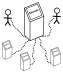
\includegraphics[scale=3]{serverrichpicture/server.pdf}
\caption{The server and the associated stations.}
\label{fig:ServerRichPicture}
\end{figure}

The stations receive the information that allows it to handle bookings done on the server.
They also have the capability of handling booking by themselves, which is then shared with the central server.
Sharing information such as the amount of available bicycles is also something the stations need to be able to do.
The dock that provide the locking/unlocking mechanism along with the bicycle detection ability have to talk to the station, for example when they need to unlock booked bicycle this information needs to be propagated from the server to the station to the individual bicycle.
This can be seen in \figref{fig:StationRichPicture}.

\begin{figure}[h]
\centering
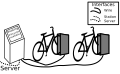
\includegraphics[scale=3]{stationrichpicture/station.pdf}
\caption{The station and the bikes.}
\label{fig:StationRichPicture}
\end{figure}

\begin{comment}
\begin{figure}[h]
\centering
\begin{subfigure}[b]{0.3\textwidth}
\centering

\includegraphics[scale=1]{Bicyclewithlock/bicylewithlock.pdf}
\caption{Locked bicycle.}
\label{fig:BicycleLocked}
\end{subfigure}
~
\begin{subfigure}[b]{0.3\textwidth}
\centering
\includegraphics[scale=1]{Bicyclewithoutlock/bicylewithoutlock.pdf}
\caption{Unlocked bicycle.}
\label{fig:BicycleUnlocked}
\end{subfigure}
\caption{Rich picture of bicycle.}
\label{fig:Bicycles}
\end{figure}
\end{comment}
	
	\chapter{Theory}
	Some background theory is needed for the development of a solution is examined and discussed.\fxnote{her skal opremses hvad vi skriver om}
	\section{Internet of Things}
This section introduces the \textbf{I}nternet \textbf{o}f \textbf{T}hings (IoT), along with examples of how it is used. 
The section also introduces various hardware considerations to provide the context in which real-world applications for the IoT are developed.

The IoT is the concept describing the interconnection of uniquely identifiable things in the problem domain.
The IoT also includes the virtual representation, the interfaces that allow for manipulation, and information retrieval regarding these things \citep{misc:InternetOfThingsDefinition, misc:InternetOfThingsDefinition2, misc:InternetOfThingsDefinition3}.

Real usage of the IoT manifests as systems to provide some service, either by informing the user about things or allowing an intelligent system to manage those things.
An example of this could be a `smart home' that allows you to use a single device to manage the connected things in your home, such as the lights or the oven in the kitchen \citep{misc:InternetOfThingsExamples}.
One society-wide use for it is the idea of a `smart power grid', where the electricity usage is monitored and managed by an intelligent system that e.g. redirects electricity if a cable has been cut somewhere in the system \citep{misc:smartGrid}.

There are already a lot of things in the IoT, and by 2020 it is estimated that there can be upwards of 26-30 billion things in it \citep{misc:IoTGrowth1,misc:IoTGrowth2}.
This likely requires a shift to the IPv6 protocol as the amount of IP addresses are severely limited by IPv4 \citep{misc:numberOfAddresses} given that the additions to IPv4, such as multiple devices sharing a single IP address, at some point becomes insufficient.

One important aspect of the things connected to the IoT is what technology they use to connect, WiFi or mobile networking are obvious choices of communication means.
For most purposes the connectivity technology has to be low-power and cheap.
Other than WiFi and mobile networking, it is possible to connect things to a server with a cable connecting to the internet, though that is not practical for things that must be mobile.
RFID chips can provide relevant information to an outside observer about the thing itself \citep{misc:rfid} with active research in making it low-cost and low-power \citep{misc:rfid2}.

The geographical location in the IoT matters, especially for sensors where the location provides important context for the accessed information \citep{misc:locationMatters}.
For example if there is a station for bicycles in a bicycle sharing system that needs to provide information regarding the amount of bicycles at the station, it is important for the usage of the information that it also provides the actual location of the station, if that is not otherwise known.

In order to give more detail on IoT, aspects about identification, communication, and software is given.

\subsection{Identification}
In order to uniquely identify the things in the IoT, different approaches can be taken.

One idea is to use the IP address of an object, which has relation to the previously discussed IPv4 versus IPv6 issue.
With IPv6, this approach would have enough addresses to uniquely identify a large number of things.
Given IPv6 has a theoretical possibility of $3.4 \cdot 10^{38}$ unique addresses \citep{misc:ipv6}, not having enough addresses would not be a problem in the foreseeable future.

When you have a unique address, you can use that to uniquely identify the given thing.
An example of use is the power grid, where each power station can uniquely be identified with the IPv6 address, and as such, in case of malfunction in one of the grid connections, it would be possible to identify the stations lacking power.

\subsection{Communication}
In order for the IoT to work, it is necessary to have a communication established.
If that was not the case, the things would not be part of the IoT, as the central idea is that you can communicate over the internet.

One idea of communication for sensors is as follows.
Each sensor has access to the internet to contact a web service with their given reading.
However, it is unrealistic that each sensor alone is directly connected to the internet, and as such, other alternatives can be performed.
One such alternative is that a thing consists of a communication device connected to several sensors and the internet.
The communication device can then read from the sensors and contact the web service.

However, the communication does not end at this point.
The idea is that the communication is not limited to machine-machine communication, but is expanded to communication over the internet, such that the things of the IoT can be contacted from anywhere on the internet.

\subsection{Software}
Examples of Software that utilise the IoT are given to get a concrete idea of the power of the IoT.

We expand on the example of the smart power grid.
Such a power grid uses the information it has about each section of the grid, to ensure that there is sufficient power reaching every part of the grid, even in cases where part of the grid malfunctions.
This ability is achieved through the system being able to automatically reroute the power flow in the grid, so power flows through functioning areas to reach the parts that would otherwise have been affected by the malfunction.

Another example is the mentioned home automation system.
For such a system, the things of the house being the lock, coffee machine, lights, washing machine etc, is then the central parts.
If the things of the house is connected to the IoT, it is possible to connect to those devices and control them over the internet.
This has several advantages, which includes ensuring the door is locked, preparing coffee before you get home, and other actions you may want to do with the things of your house, even though you are at work or on vacation.
	
	\afterpage{\thispagestyle{empty}}

	\bibliography{Bibliography}
	
	\label{lastpagewithoutappendix}

	\appendix
	%\input{Src/Appendix/File}
	
	\cleardoublepage
	\phantomsection
\end{document}
